\documentclass{article}
\usepackage[utf8]{inputenc}
\usepackage{tikz}
\usetikzlibrary{shapes,arrows}
\usepackage[ruled,vlined]{algorithm2e}
%\usepackage{algpseudocode}
\usepackage{multicol}
\renewcommand{\contentsname}{{\Huge Table de Matières}}
\usepackage{titlesec}
\usepackage{xcolor}
\usepackage{graphicx}
\titleformat{\section}{\huge\bfseries}{\thesection}{1em}{}
\titleformat{\subsection}{\LARGE\bfseries}{\thesubsection}{1em}{}
\titleformat{\subsubsection}{\Large\bfseries}{\thesubsubsection}{1em}{}
\begin{document}
%first page
\begin{center}
\pagenumbering{gobble}
\linespread{2.0}\selectfont

{\Huge U}{\huge NIVERSITÉ DE }{\Huge M}{\huge ONTPELLIER}\\
{\huge L2}{\LARGE ~INFORMATIQUE }
\\~\\~\\~\\~\\
{\Large\textbf{GOLF MATHÉMATIQUE}}
\\~\\~\\~\\~\\

\linespread{1}\selectfont

RAPPORT DE PROJET T.E.R\\
PROJET INFORMATIQUE HLIN405\\
\vfill
\end{center}
\begin{multicols}{2}
\begin{flushleft}
\textbf{Etudiants:}\\
~~M. Mike Germain\\
~~M. Benjamin Baska\\
~~M. Kevin Lastra
\end{flushleft}
\columnbreak
\begin{flushright}
\textbf{Encadrante:}\\
~~Mm. Annie Chateau
\end{flushright}
\end{multicols}
\newpage
%bilan
\pagenumbering{arabic}
\setcounter{page}{1}
\tableofcontents
\newpage
%introduction
{\textbf{\Huge Introduction}}\\~\\~\\
~~Sous la direction de Mm. Annie Chateau, notre groupe composé de Mike Germain, Benjamin Baska et Kevin Lastra à travaillé sur le développement du jeux "Golf Mathématique" comme projet du module HLIN405.

\newpage
%cahier de charges
\section{Organisation du projet}
\subsection{Objectifs et cahier des charges}
~\\~\\
wtf
\\~\\
\textbf{\large Base et Règles}
\\~\\
aucune idée 
\\~\\
\textbf{\large Interface Graphique}
\\~\\
pire
\\~\\
\textbf{\large Génération automatique de la carte}
\\~\\
x2
\\~\\
\textbf{\large Intelligence Artificielle}
\\~\\
au secours
\\~\\
\subsection{Division du travail}
\tikzstyle{decision} = [diamond, draw, fill=blue!20, 
    text width=4.5em, text badly centered, node distance=3cm, inner sep=0pt]
\tikzstyle{block} = [rectangle, draw, fill=blue!20, 
    text width=5em, text centered, rounded corners, minimum height=4em]
\tikzstyle{line} = [draw, -latex']
\tikzstyle{cloud} = [draw, ellipse,fill=red!20, node distance=3cm,
    minimum height=2em]

\begin{figure}[h]
\centering
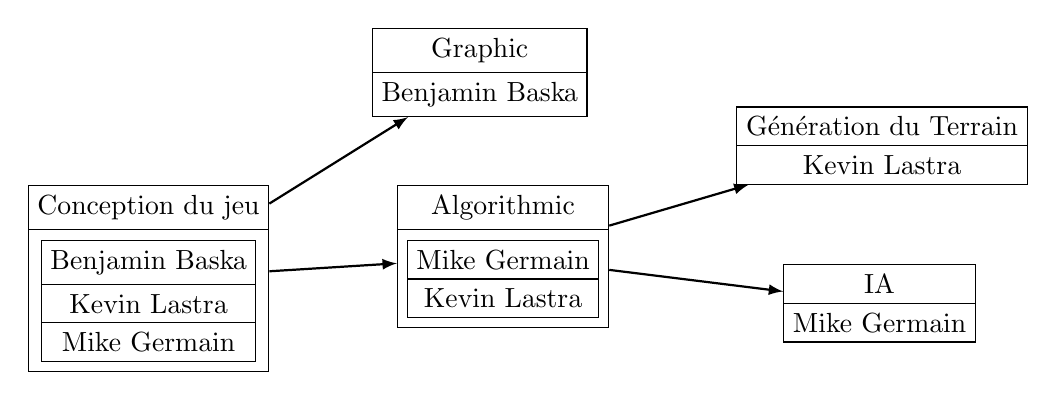
\begin{tikzpicture}[
					double/.style={draw, anchor=text, rectangle split, rectangle split parts=2},
					triple/.style={draw, anchor=text, rectangle split, rectangle split parts=3}]
    % Place nodes
    \node [double] (A) at (-5,0){Conception du jeu
    	\nodepart{second}
    	\tikz{
    		\node[triple]{Benjamin Baska
    		\nodepart{second}Kevin Lastra
    		\nodepart{third}Mike Germain
    		};
    	}
    };
    \node [double] (B) at (0,2){Graphic
    	\nodepart{second}
    	Benjamin Baska
    };
    \node [double] (C) at (0,0){Algorithmic
    	\nodepart{second}
    	\tikz{
    		\node[double]{Mike Germain
    		\nodepart{second}Kevin Lastra
    		};
    	}
    };
	\node [double] (D) at (5.5,-1){IA
    	\nodepart{second}
    	Mike Germain
    };
    \node [double] (E) at (4,1){Génération du Terrain
    	\nodepart{second}
    	Kevin Lastra
    };
    \draw[thick,-latex] (A) edge (B);
    \draw[thick,-latex] (A) edge (C);
    \draw[thick,-latex] (C) edge (D);
    \draw[thick,-latex] (C) edge (E);
    % Draw edges
    
\end{tikzpicture}~\\
\caption{Diagramme de répartition du travail.}

\end{figure}
\newpage
\subsection{Outils de travail}
\textbf{\large Langage de programmation}\\
Le langage qu'on à choisi pour le développement du jeux, est le C++ pour 2 raisons principales:

\begin{enumerate}
\item Ce langage est un langage de "programmation orienté aux objets" (POO).
\item Grace aux modules de HLIN202 et HLIN302 on a une base de connaissance avec laquelle on peut travailler de manière très confortable.
\end{enumerate}
\textbf{\large Software de programmation graphique}\\
On a choisit la librairie QT pour les différents avantages qu'elle nous apporte. Cette librairie dispose d'une bonne documentation, elle é adapté au langage C++ et elle dispose aussi d'un outil de travail très intéressant appelé "QT Creator", qui rend le travail plus facile.\\~\\
\textbf{\large Travail collaboratif}\\
Nous avons utilisé de multiples programmes:
\begin{enumerate}
\item GitHub. Ce logiciel nous permet de partager les avancements du travail réalisé par chacun depuis différents ordinateurs et aussi de sauvegarder plusieurs versions du travail, ce qui est très rassurant en cas de perte.
\item Discord. Ce logiciel nous permet le partage d'écran, la communication orale et écrit, ce qui est très utile pour le développement du jeux.
\end{enumerate}
\textbf{\large Éditeur de texte}\\
La production du projet est réalise grâce a plusieurs éditeur de text:
\begin{enumerate}
\item Éditeur de code -
Emacs, sublime et QTCreator.
\item Éditeur \LaTeX{} - TexMaker
\end{enumerate} 
\newpage
\section{Conception}
De la premier réunion, utilisant l'image proportionnée dans le sujet du projet, on à travaillé dans une architecture, pour le quel ce jeux s'adapterait mieux.\\~\\
La premier chose qu'on à définit est la structure du terrain de jeux, Terrain de NxM Node, après la classe Terrain crée on a structuré une classe qui manipulerait tout les entre/sortie ("GameMaster") et finalement les joueur avec une classe "PlayerController".\\~\\
% Define block styles
\tikzstyle{decision} = [diamond, draw, fill=blue!20, 
    text width=4.5em, text badly centered, node distance=3cm, inner sep=0pt]
\tikzstyle{block} = [rectangle, draw, fill=blue!20, 
    text width=5em, text centered, rounded corners, minimum height=4em]
\tikzstyle{line} = [draw, -latex']
\tikzstyle{cloud} = [draw, ellipse,fill=red!20, node distance=3cm,
    minimum height=2em]
\begin{figure}[h]
\centering
\begin{tikzpicture}[node distance = 2cm, auto]
    % Place nodes
    \node [block] (OP) {Out Put};
    \node [block, below of=OP] (GM) {Game Master};
    \node [block, right of=GM, yshift=0cm, xshift=2cm] (Ter) {Terrain};
    \node [block, right of=Ter, yshift=0cm, xshift=2cm] (init) {Node};
    \node [block, below of=GM] (PC) {Player Controller};
    \node [block, below of=init] (IA) {Intelligence Artificial};
    \node [cloud, right of=PC, yshift=-0.5cm, xshift=1cm] (A) {if IA};
    % Draw edges
    \path [line] (init) -- node[near start]{1} node[near end]{[*..,*.]}(Ter);
    \path [line] (Ter) -- (GM);
    \path [line] (GM) -- (Ter);
    \path [line] (GM) -- (OP);
    \path [line] (PC) -- (GM);
    \path [line,dashed] (PC) -- (A);
    \draw [line,dashed] (A) -- (IA);
    \draw [line,dashed] (IA) -- node[above]{send request}(PC);
    \draw [line,dashed] (A) -- node[near start]{else} ++ (-2,0) --++(0,4) -- (OP);
    \draw [line,dashed] (OP) --++ (2.5,-1.2) --++ (0,-1.8) --++ (1,-0.5);
\end{tikzpicture}~\\
\caption{Représentation du flux du jeu.}
\end{figure}
\subsection{Base du jeu}
Golf mathématique est un sous type du golf original, donc cela signifie qu'on doit modifier le jeu sont perd l'esprit du golf.
Le Golf est un jeux de plusieurs joueur par tour, la personne qui gagner est celui qui a moins de points, etc...
Donc pour définir les bases de notre jeu on doit utiliser les règles du jeu original et les objets qui lui entour.
Dans un Terrain de golf, on a un:
\begin{itemize}
\item Départ(zone ou les jouer commence.)
\item Cible(le trou)
\item Obstacles(zone d'eau ou sable)
\end{itemize}
Un joueur peut avoir plusieurs position et tape la balle avec une portée.
Avec tous ça on trouve des éléments avec le quelle on peut travailler.
Un terrain on l’interprétera comme un tableau d'entier les quelles la valeur sera la portée de la balle.
Un terrain sera divise on 3 zones différents:
\begin{itemize}
\item Eau
\item sable
\item Herbe
\end{itemize}
\subsection{Graphic}
\subsection{Intelligence Artificielle - IA}
\newpage
\subsection{Génération du Terrain}
\subsubsection{Génération Automatique}
Pour générait un terrain de manière automatique on doit place des règles:
\begin{itemize}
\item Le Terrain doit être connexe ou au moins cheminable.
\item La génération des portée doit être presque linéal.

\end{itemize}
Après avoir testé différents idées, nous avons trouvé une solution très convenable pour construire un terrain. Pour générait notre terrain on va produire un chemin est sur celui la on va faire apparente la surface.\\
Cette algorithme est divise en deux passage sur une grille:\\~\\
\textbf{\Large{Premier Passage}}\\
On produit un premier point de manière aléatoire ($P_{x,y}$), et à partir de ce point on génère n-1 autres points ($P_{x,y}$,...,$Pn_{x_n,y_n}$).
\begin{center}
	$k\leq$ n et $k>0, P_{k} = P_{k-1} + \lambda(a, b)$
\end{center}
Telle que le vecteur (a, b)$\in$V, avec V l'ensemble des 7 différents directions valides représente avec des vecteurs.
\begin{center}
	V=\{(-1,-1),(-1,0),...,(1,1)\}\\
	Et $\lambda = B_i$ avec B = \{n-1,n-1,n-2,n-3,...,4,3,2,2\}.
\end{center}
Avec cette algorithme ont trouverait que:\\~\\
X:"l'ensemble des terrains générés" \\
Y:"l'ensemble des chemins possibles"\\
\(\forall x \in X, \exists y \in Y\) telle que "y" est un chemin valide.\\~\\
Avec cette phrase on pouvais générer le terrain sans avoir a penser aux possibles contraintes comme la connexité.
\newpage
\textbf{\Large{Pseudo Code}}\\~\\
\begin{algorithm}[H]
	\caption{GénérationChemin(d lo: entier, d la: entier,d n: entier): Tableau d'entier}
	\SetKwInOut{Parameter}{variables}
	\SetKwInOut{Debut}{début algorithme}
	\SetKwData{I}{i}\SetKwData{LO}{lo}\SetKwData{LA}{la}
	\SetKwData{DIR}{dir}\SetKwData{Va}{v.x}\SetKwData{Vb}{v.y}
	\SetKwData{V}{v}
	\SetKwArray{TAB}{Tab}\SetKwData{N}{n}
	\SetKwFunction{Random}{random}\SetKwFunction{GDIR}{getdirection}
	\SetKwFunction{NPOS}{nouvelPosition}	
	\Parameter{Tab: tableau d'entier bidimensionnel de taille n*m.\\
	i: entier.\\
	v: structure vecteur contenant une paire d'entier\\ "x" et "y".}
	\Debut\\
	\BlankLine
	\I $\leftarrow 1$\;
	\tcp{on définit v le premier point du chemin.}
	\Va $\leftarrow$ \Random{}$\%$($\frac{lo}{2}$)\;
	\Vb $\leftarrow$ \Random{}$\%$($\frac{la}{2}$)\;
	\TAB{\Va}$[$\Vb$]$ $\leftarrow$ 1\;
	\While{\I $<$ \N}
	{
		\DIR $\leftarrow$ \GDIR{}\;\tcp{renvoi un nombre entre {0-7} aléatoirement, qui représente les 8 diffèrent directions}
		\V $\leftarrow$ \NPOS{\V ,\DIR}\;\tcp{renvoi un vecteur qui représente la nouvel position $v_{n+1}$ par rapport a la direction et la position $v_{n}$;}
		\If{\V est valide $\&\&$ \TAB{\Va}$[$\Vb$]$ $==$ 0}
		{
			\TAB{\Va}$[$\Vb$]$ $\leftarrow 1$\;
		}
	}
	\Return \TAB\;
\end{algorithm}
~\\~\\
\newpage
Cette algorithme va nous rendre un tableau d'entier, le quelle on peut représente avec un graph:\\
GénérationTerrain(n,m,5);\\
\begin{figure}[h]
\centering
\begin{tikzpicture}
%nodes
\node [draw, rectangle,label = "Terrain"
		,minimum size = 3cm] (map) 
{
\begin{tikzpicture}
	\foreach \point [count=\i] in {(-5,4),(-4,5.2),(-3,4),(-2,2.5),(-3,1)}
	{
	\fill \point circle (2pt);
	\draw[black, thick] \point circle (1cm);
	\draw[red] \point+(0,0.5) node {$\i$};
	}
\end{tikzpicture}
};
\end{tikzpicture}~\\
\caption{les cercles représente la zone ou le Terrain va ce générait.Anexe 0.}
\end{figure}
\newpage
\definecolor{color1}{RGB}{166,65,180}
\definecolor{color2}{RGB}{55,91,3}
\textbf{\Large{Deuxième Passage}}\\
Déjà générait le chemin, on va passer case par case de notre grille et on va teste si la distance entre la case est un point du chemin est inférieur a un certain nombre.
\begin{center}
On pose (x, y) une case.\\
T l'ensemble des points du chemin.\\
$\lambda$ le rayon.\\
Si distance((x, y), $T_i$) $< \lambda$ alors la case est valide.
\end{center}
si une case est valide ça veut dire que cette case est partie de la surface de notre terrain, donc on doit lui donne une porté, cette porté est définit par la formule suivant:
\begin{center}
	porté = {\color{color1}$(2 + (\frac{dist*8}{sranyon}\%8))$} + 
	{\color{color2}$(((rand()\%5)-2)\%2)$}
\end{center}
Cette formule est divisé on 2 partie, représente par les couleur:
\begin{center}
	1.~~~~~ $(2 + (\frac{dist*8}{sranyon}\%8))$
\end{center}
\textbf{dist} est la distance entre le dernier point du chemin et la case actuel.\\
\textbf{srayon} est la distance entre le dernier point du chemin et le point valide le plus éloigner du dernier point du chemin.\\
A l'aide de GeoGebra on peut représenter cette formule de manière plus graphic.\\
\begin{figure}[!h]
\centering
 \includegraphics[scale=0.5]{Images/Geogebraimg1.png}\\
 \caption{srayon $=$ 20, 9 au lieu 8 et 1 au lieu 2. La portée d'un point est équivalent a l'axe z.}
\end{figure} 
\begin{center}
	2.~~~~~ $(((rand()\%5)-2)\%2)$\\
\end{center}
rand() un nombre aléatoire entre 0 et RAND{\_}MAX(un nombre très grand qui dépens du langage);
\begin{center}
 $rand()\%5 \leftarrow$ est un nombre entre 0 et 4\\
 $((rand()\%5)-2) \in\{-2,-1,0,1,2\}$\\~\\
 3 nombre pair(60$\%$) et 2 nombre impair(40$\%$).\\~\\
 $(((rand()\%5)-2)\%2) \in\{-1,0,1\}$,\\~\\
\end{center}
ça veut dire qui est plus probable d'avoir 0 que 1 ou -1 donc 60$\%$ de probabilité de ne pas modifier et 40$\%$ pour modifier.

\begin{center}
\textbf{\Large{Pseudo Code}}
\end{center}
\begin{algorithm}[H]
	\caption{GénérationTerrain(d Tab: tableau d'entier,d Ch:tableau de vecteur(les points du chemin),d lo:entier,d la:entier): Tableau d'entier}
	\SetKwInOut{Parameter}{variables}
	\SetKwInOut{Debut}{début algorithme}
	\SetKwData{X}{x}\SetKwData{LO}{lo}\SetKwData{LA}{la}
	\SetKwData{Y}{y}\SetKwArray{CH}{Ch}\SetKwData{EXT}{ext}
	\SetKwArray{TAB}{Tab}
	\SetKwFunction{Random}{random}\SetKwFunction{INRAD}{dansRayon}
	\SetKwFunction{FEXTREM}{extrem}	\SetKwFunction{PORTEE}{calcPortee}	
	\Parameter{}
	\Debut\\
	\BlankLine
	\EXT $\leftarrow$ \FEXTREM{\TAB}\;
	\tcp{renvoi le point le plus éloigner du dernier point du chemin(Ch[n-1]).}
	\For{$\X \leftarrow 0$ \KwTo \LO}
	{
		\For{$\Y \leftarrow 0$ \KwTo \LA}
		{
		\BlankLine
			\If{\INRAD{\TAB{\X}$[$\Y$]$,\CH} et \TAB{\X}$[$\Y$]$ $\notin$ \CH}
			{
				\tcp{dansRayon renvoi vrai ou faux dépendant si un point (x, y) est dans le rayon d'un point du chemin.}
				\TAB{\X}$[$\Y$]$ $\leftarrow$ \PORTEE{\EXT ,\CH{n-1},\TAB{\X}$[$\Y$]$}\;
				\tcp{calcPortee renvoi la porte d'un point utilisant la formule vue avant.}
			}
		}
	}
	\Return \TAB\;
\end{algorithm}
\begin{center}
\begin{tikzpicture}
%nodes
\node [draw, rectangle,label = "Terrain"
		,minimum size = 3cm] (map) 
{
\begin{tikzpicture}
	\foreach \point [count=\i] in {(-5,4),(-4,5.2),(-3,4),(-2,2.5),(-3,1)}
	{
	\draw[black, fill] \point circle (1.5cm);
	}
\end{tikzpicture}
};
\end{tikzpicture}~\\
figure 0: les zones noire représenter la surface jouable.Anexe 0.
\end{center}
\newpage
\section{Bibliographie}
\section{Annexes}
\end{document}